%! TEX root = main.tex

The first benchmark is done with the 2D Taylor-Green vortex (TGV) problem described in section \ref{sec:petibm-vv}.
This TGV problem serves as a good benchmark case because it reduces the number of required residual constraints in PINNs.
The approach described in section \ref{sec:periodic-boundary} eliminates the constraints coming from periodic BCs.
The optimization becomes simpler, and the optimizer can focus only on IC and PDE residuals.

The neural network used in the PINN solver is the weight-normalized MLP described in section \ref{sec:mlp}.
Cases in this benchmark can be categorized into five groups.

Cases in the first group use common optimization configurations (described later).
They serve as the base for all tests in the subsequent subsections for comparison.
This category covers different numbers of hidden layers ($N_l$), numbers of neurons per hidden layer ($N_n$), and numbers of training points per batch ($N_{bs}$).
$N_l$ ranges from $1$ to $3$ layers.
$N_n=2^i$ for $i$ ranging from $4$ to $8$.
$N_{bs}=2^i$ for $i$ ranging from $10$ to $16$.
This group contains a total of 105 cases.

The other four groups will be described in the corresponding subsections: section \ref{sec:pinn-2d-tgv-scaling} describes cases for parallel scaling tests; section \ref{sec:pinn-2d-tgv-training-strategy} describes cases with adaptive loss aggregation, cases with cyclical learning rates and SWA, and cases with conjugate-gradient solvers.

The training processes for cases in the first group are the same: 400,000 iterations of the Adam optimization with an exponentially-decaying learning rate schedule: $\operatorname{lr}(k) = 0.95^\frac{k}{5000}$, where $k$ is the iteration counter.
We use the default parameters for the Adam optimizer from PyTorch: $\beta_1=0.9$, $\beta_2=0.999$, and $\epsilon=10^{-8}$.

Given an $N_{bs}$, a total of $10,000 \times N_{bs}$ points are used to evaluate PDE residuals.
And another $10,000 \times N_{bs}$ points are used to evaluate IC residuals.
In other words, each batch of training points is repeated every $10,000$ iterations.
And the models see each training point $40$ times during the training process.

The training points for PDE residuals are randomly sampled from the spatial-temporal domain of $[-\pi, \pi]\times[-\pi, \pi]\times(0, 100]$.
Note that $t=0$ is excluded from the sampling pool.
It means the PDE is not enforced at t=0.
The training points for IC residuals are randomly sampled from the spatial domain of $[-\pi, \pi]\times[-\pi, \pi]$ and have a fixed time $t=0$.

The hardware used is NVIDIA's V100 GPUs.
All cases in the first group ran on only one GPU.

After training, the PINN solver's prediction errors (i.e., accuracy) were evaluated on cell centers of a $512 \times 512$ Cartesian mesh against the analytical solutions.
And if needed, we predicted solution snapshots at $t=0, 1, 2, \cdots, 100$ for temporal errors.
Two types of errors were used: spatial-temporal error ($L_{2,sp-t}$), and spatial $L_2$ error at a given time $t$.
$L_{2,sp-t}$ has been defined in \eqref{eq:spt-err-def}.
The $L_2$ error norm for a given $t$ is
\begin{equation}\label{eq:l2norm}
    \begin{aligned}
        L_2
        &=
        \sqrt{
            \frac{1}{L_x L_y}
            \int\limits_{x}\int\limits_{y} \lVert f - f_{ref}\rVert^2
            \diff x \diff y
        } \\
        &\approx
        \sqrt{
            \frac{1}{N_x N_y}
            \sum\limits_{i}^{N_x}\sum\limits_{j}^{N_y}
            \left(f^{\left(i, j\right)}-f_{ref}^{\left(i, j\right)}\right)^2
        }
    \end{aligned}
\end{equation}
$i$ and $j$ are the indices of a cell center in the Cartesian mesh.
For this particular TGV benchmark, $N_x=N_y=512$, and $L_x=L_y=2\pi$.

A special note should be made here: the PINN solver used single-precision floats, which is the default for modern deep learning frameworks like PyTorch and TensorFlow.

To have a comparison against conventional CFD code, figure \ref{fig:petibm-tgv-spatial-temporal-error} shows the $L_{2,sp-t}$ versus time-to-solution in seconds.
\begin{figure}[hbt!]
    \centering%
    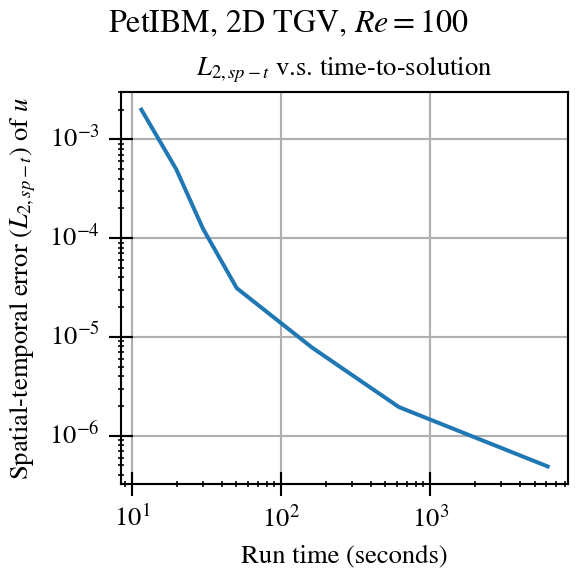
\includegraphics{tgv-2d-re100/petibm/tgv-2d-re100-err-u}%
    \caption[%
        PetIBM, TGV 2D $Re=100$: spatial-temporal error ($L_{2,sp-t}$) of $u$%
    ]{%
        PetIBM, TGV 2D $Re=100$: spatial-temporal error ($L_{2,sp-t}$)  of $u$ versus time-to-solution in seconds%
    }\label{fig:petibm-tgv-spatial-temporal-error}%
\end{figure}
We will be able to compare the time cost to get the desired error with conventional CFD code and with a PINN solver.
The configurations of PetIBM simulations can be found in section \ref{sec:petibm-vv}.
% vim:ft=tex
